\chapter{遺伝的アルゴリズム}
本章では,担当割り振り決定手法で使用した遺伝的アルゴリズムについて説明する.
\section{概要}
遺伝的アルゴリズム(Genetic Algorithm; GA)は,1975年にミシガン大学のJohn Hollandが提案した,生物が環境に適応して進化する過程を工学的に模倣した最適解探索アルゴリズムである.問題の解を生物の個体として表現し,解の良さを表す適応度を算出して評価する.複数個体の中から適応度が高い個体の遺伝子が引き継がれるように,選択,交叉,突然変異を繰り返し,各世代の個体集団を生成する.終了条件には,世代交代数などが用いられる.終了条件を満たすと,最終世代の最良個体を出力し,処理を終了する.GAの基本アルゴリズムを図\ref{03001}に示す.


\section{染色体表現}
GAでは,個体の形質を規定する値を遺伝子,複数の遺伝子の集まりを染色体,染色体上の遺伝子の位置を遺伝子座と呼ぶ.染色体の例を図\ref{03002}に示す.

\begin{figure}[htbp]
\begin{center}
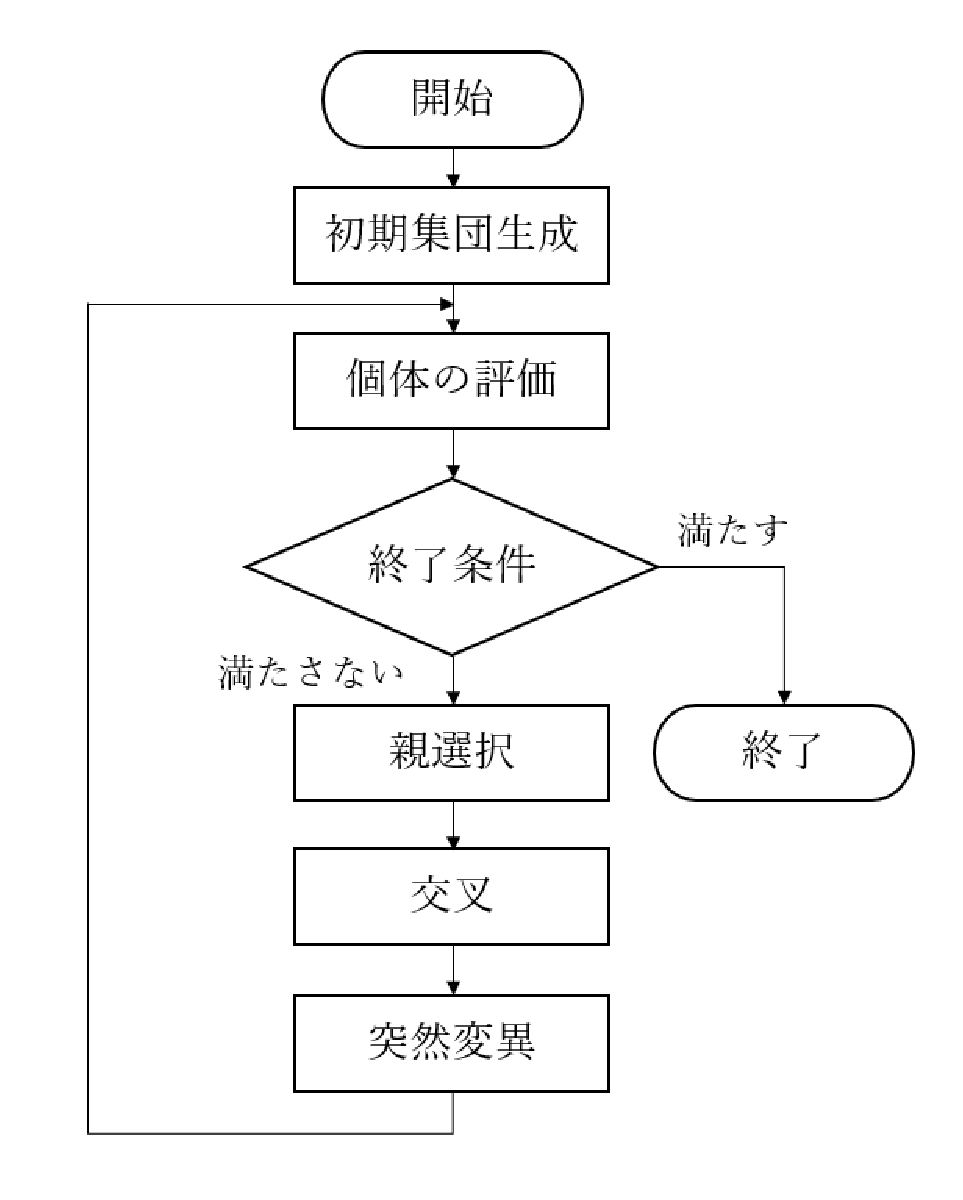
\includegraphics[scale=0.5]{image/GA/03001.eps}
\caption{GAの基本アルゴリズム}
\label{03001}
\end{center}
\end{figure}

\begin{figure}[htbp]
\begin{center}
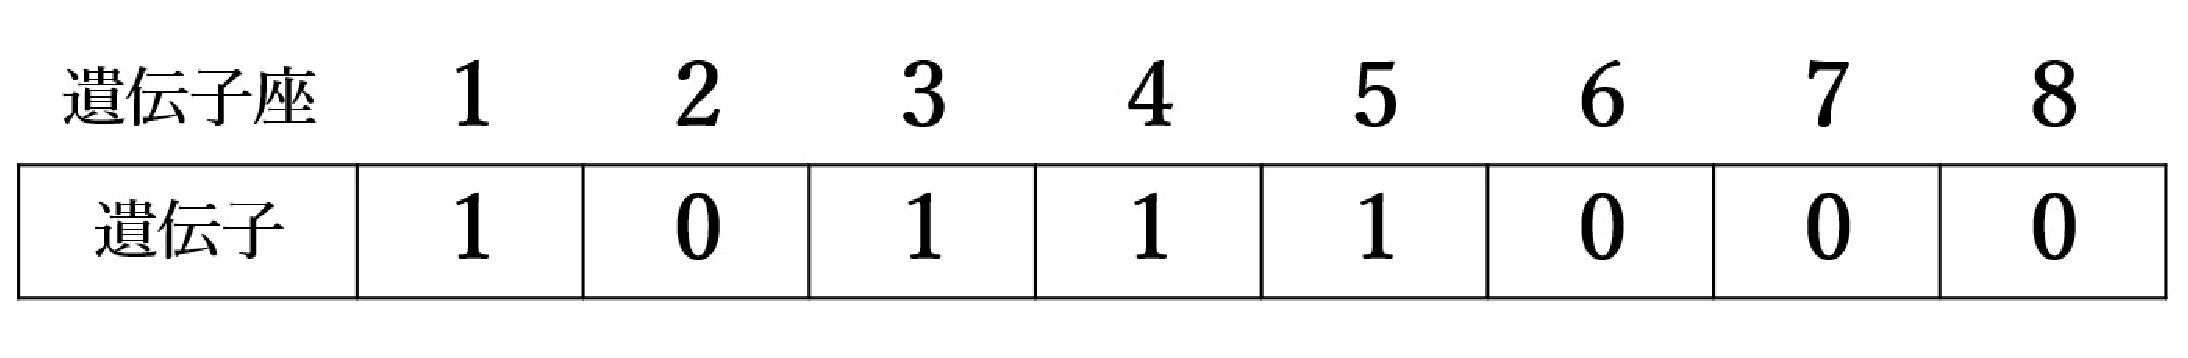
\includegraphics[scale=0.3]{image/GA/03002.eps}
\caption{染色体の例}
\label{03002}
\end{center}
\end{figure}

\section{親個体の選択}
GAでは,個体集団から親となる2個体を選択し,次世代の子個体を生成する.より良い適応度の個体ほど選択される確率を高くする必要がある.親個体の選択方法には,ルーレット選択,ランキング選択,トーナメント選択などがある.ルーレット選択は,各個体の適応度に基づいて選択確率を決定する方法である.各個体の適応度が一様になるほど,最良個体が選択されにくくなるという問題点がある.ランキング選択は.適応度に応じて各個体の順位を決定し,事前に設定した選択確率によって親個体を選択する方法である.ルーレット選択とは異なり,個体の順位によって選択確率を決定できるため,各個体の選択確率が一様になることを避けることができる.トーナメント選択は,個体集団から一定数の個体をランダムに選択し,最も適応度の高いものを親個体とする方法である.個体集団から選択する個体数によっては,適応度の低い個体でも次世代に残る可能性が高いため,収束しにくくなる恐れがある.

\section{交叉と突然変異}
交叉は,選択された2つの親個体から子個体を生成する操作である.交叉の方法には,一点交叉や多点交叉,一様交叉などがある.一点交叉は,ランダムに交叉点を1つ選択し,交叉点の前後の遺伝子列を交換して子個体の染色体とする.多点交叉は,交叉点を複数選択し,一点交叉と同様に処理する.一様交叉は,ランダムに遺伝子座を選択し,遺伝子ごとに交換するかを決定する.

突然変異は,一定の確率で,親個体に存在しない遺伝子を子個体に持たせる操作である.突然変異によって親個体とは異なる特徴を獲得できるため,局所解への収束を避けることができる.しかし,親個体が持っていた良い遺伝子を失う可能性があるため,突然変異を起こす確率を適切に設定する必要がある.